%% 
%% Skript Differentialgeometrie im Wintersemester 12/13
%% Zur Vorlesung von Dr. Grensing am KIT Karlsruhe
%% 
%% Kapitel 9
%% 
\chapter{Jacobifelder}

F"ur $p,q \in M$ sei $\Omega_{pq}$ der Raum aller glatten Kurven
$c:[0,1] \to M$ mit $c(0)=p$ und $c(1)=q$.
\begin{center}\begin{tikzpicture}[font=\scriptsize]
    %	\tikzgitter{(-5,-5)}{(5,5)} % Hilfsgitter

    \coordinate (p) at (-3.5,-1); \coordinate (q) at ($-1*(p)$); \fill
    (p) circle(0.05)node[left]{$p$} (q) circle(0.05)node[right]{$q$}
    (0,0) circle(0.05)node[below right]{$c$};

    \coordinate (ctrl) at (2,-0.25); \draw (p) ..controls(p) and
    ($-1*(ctrl)$).. (0,0) ..controls(ctrl) and (q).. (q);

    \coordinate (a) at (0,-1); \coordinate (b) at ($-1*(a)$);
    \coordinate (ctrl2) at (0.25,0.5); \draw (a) ..controls(a) and
    ($-1*(ctrl2)$).. (0,0) ..controls(ctrl2) and (b).. (b); \draw[->]
    (0,0) -- ($2*(ctrl2)$) node[right]{$\difffrac{}{s}c_s$};

    \def\faktor{0.2} \foreach \y in {1, 2}{ \path (a) ..controls(a)
      and ($-1*(ctrl2)$).. (0,0) ..controls(ctrl2) and
      (b).. coordinate[pos=\y * \faktor] (coord) (b);
      % \draw[red] (coord) circle(0.05);
      \draw[dashed] (p) ..controls(p) and ($(coord)
      -1*(ctrl)$).. (coord) ..controls($(coord) + (ctrl)$) and
      (q).. (q); } \foreach \y in {1, 2, 3}{ \path (a) ..controls(a)
      and ($-1*(ctrl2)$).. coordinate[pos=1 - \y * \faktor] (coord)
      (0,0) ..controls(ctrl2) and (b).. (b);
      % \draw[red] (coord) circle(0.05);
      \draw[dashed] (p) ..controls(p) and ($(coord)
      -1*(ctrl)$).. (coord) ..controls($(coord) + (ctrl)$) and
      (q).. (q); }
  \end{tikzpicture}\end{center}

\begin{Dfn}
  Eine \CmMark[Variation]{(glatte) Variation} einer glatten Kurve
  $c:[a,b] \to M$ ist eine glatte Abbildung
  \begin{align*}
    h:(-\epsilon, \epsilon) \X [a,b] \to M && h_s(t) = h(s,t)
  \end{align*}
  mit $h_0 = c$. Gilt $h(\cdot, a) \equiv c(a)$ und $h(\cdot, b)
  \equiv c(b)$, so hei"st $h$ eine \CmMark[Variation!mit festen
  Endpunkten]{Variation mit festen Endpunkten} oder
  \CmMark[Variation!eigentliche]{eigentliche Variation}. Man schreibt
  $c_s$ f"ur eine Variation $h$ von $c$.
\end{Dfn}

Ist $c_s$ eine glatte Variation von $c$, so ist
\begin{align*}
  Y(t) &= \difffrac[s=0]{}{s} c_s(t)\\
  &= \difffrac[s=0]{}{s} h(s,t) =
  h_{*(0,t)}\left(\pdifffrac{}{s}\right)
\end{align*}
ein Vektorfeld entlang $c$. ist $c_s$ eigentlich, so gilt $Y(a) = 0
\in \T_{c(a)}M$ und $Y(b) = 0 \in \T_{c(b)}M$.
\begin{center}\begin{tikzpicture}[font=\scriptsize]
    \coordinate (1) at (-2,-1); \coordinate (2) at (0,0); \coordinate
    (3) at (2,1.5); \coordinate (ctrl) at (1.5,0.25); \draw (1)
    ..controls(1) and ($-1*(ctrl)$)..node[pos=0.6,below]{$c$}
    coordinate[pos=0.9] (a) (2) ..controls(ctrl) and (3)..  (3); \fill
    (a) circle(0.05); \draw[->] (a) -- ($(a) + (0.5,1)$)
    node[left]{$Y(t)$};
  \end{tikzpicture}\end{center}
Tats"achlich ist jedes Vektorfeld ein solches Variationsfeld einer
Variation von $c$: Ist $Y$ ein Vektorfeld entlang $c$, so definiert
$h(s,t) = \exp_{c(t)}(s Y(t))$ eine Variation von $c$ und es gilt:
\begin{align*}
  \difffrac[s=0]{}{s} h(s,t) &= \exp_{c(t)*0}(Y(t))\\
  &= \id_{\T_{c(t)}M}(Y(t)) = Y(t).
\end{align*}
Falls $Y$ in den Endpunkten von $c$ verschwindet, so ist die so
definierte Variation eigentlich. Bestimme $\difffrac[s=0]{}{s} E(c_s)$
und $\difffrac[s=0]{}{s}\calL(c_s)$:
\begin{align*}
  \frac{1}{2} \difffrac[s=0]{}{s} \langle \dot c_s, \dot c_s \rangle &= \langle \nabla_s \dot c(s), \dot c(s) \rangle\\
  &= \left\langle \nabla_s \difffrac{}{t} c_s, \dot c(s) \right\rangle = \left\langle \nabla_t \difffrac{}{s} c_s, \dot c_s \right\rangle \\
  &= \left\langle \difffrac[s=0]{}{s} c_s, \dot c_s \right\rangle' - \left\langle \difffrac[s=0]{}{s} c_s, \nabla_t \dot c_s \right\rangle \\
  &= \left\langle Y, \dot c \right\rangle' - \left\langle Y, \nabla_t \dot c \right\rangle\\
\end{align*}
\begin{align*}
  \difffrac[s=0]{}{t} \|\dot c_s\| &= \frac{1}{2 \|c_s\|} \difffrac[s=0]{}{s} \langle \dot c_s, \dot c_s \rangle\\
  &= \frac{\langle Y, \dot c \rangle' - \langle Y, \nabla_t \dot c
    \rangle}{\|\dot c\|}
\end{align*}
Damit folgt:
\begin{align*}
  \difffrac[s=0]{}{s} E(c_s) = \difffrac[s=0]{}{s} \int_a^b
  \frac{1}{2} \|\dot c_s\| = \left. \langle Y, \dot c \rangle
  \right|_a^b - \int_a^b \langle Y, \nabla_t \dot c \rangle
\end{align*}
Betrachte $E: \Omega_{pq} \to \R$. Dann ist $c \in \Omega_{pq}$ genau
dann eine Geod"atische, wenn $c$ ein kritischer Punkt von $E$ ist, das
hei"st $\difffrac[s=0]{}{s}E(c_s) = 0$ f"ur jede eigentliche Veriation
von $c$.  Ist $c$ ein kritischer Punkt von $E$, so sei $c_s$ die von
$Y = f \nabla_t \dot c$ mit $f(0) = 0 = f(1)$ erzeugte Variation.
Dann ist $c_s$ eigentlich und es gilt
\begin{align*}
  0 = \difffrac[s=0]{}{s} E(c_s) = - \int_a^b f \|\nabla_t \dot c\|^2
\end{align*}
also $\nabla_t \dot c = 0$.  Ist $c$ nach der Bogenl"ange
parametrisiert, so gilt
\begin{align*}
  \difffrac[s=0]{}{s} \calL(c_s) = \difffrac[s=0]{}{s} E(c_s)
\end{align*}
%% 
%% Vorlesung <2013-1-11 Fri>
%% 
Eine kurve $c \in \Omega_{pq}$ ist genau dann ein kritischer Punkt von
$\calL$, wenn $c$ eine umparametrisierte Geod"atische ist.

\section{Ausblick: Hesse \& Morse - Theorie}

Sei $f \in C^\infty(M)$, sei nach Konvention $\nabla_X f = X(f) = \dop
f(X)$, und $\nabla f = \dop f \in \Omega^1(M) = \Gamma(\T M^*)$. F"ur
die Hessesche $\Hh_f = \nabla^2 f$ gilt nach Proposition
\ref{prop-7-3}:
\begin{align*}
  \nabla^2 f (X,Y) &= (\nabla_X \dop f)(Y) = X(\dop f(Y)) - \dop f(\nabla_X Y)\\
  &= X(Yf) - (\nabla_X Y)(f) \qquad (= \nabla_{X,Y}^2 \text{ in Kapitel 7})\\
  &= [X,Y]f + Y(Xf) - (\underbrace{\nabla_X Y - \nabla_Y X}_{\mathclap{[X,Y] \text{ Torsionsfreiheit}}}) f - (\nabla_Y X) f\\
  &= Y(Xf) - (\nabla_YX)(f) = \nabla^2 f(Y,X) = \Hh_f(Y,X)
\end{align*}
Die Hessesche ist also eine symmetrische $\R$-Bilinearform $\Hh_f:
\calV(M) \X \calV(M) \to C^\infty(M)$. Sie ist im Allgemeinen
\emph{nicht} $\C^\infty(M)$-bilinear. Ist $p \in M$ ein kritischer
Punkt von $f$, das hei"st $\dop f|_p = 0$, dann h"angt $\Hh_f|_p$ nur
von $\xi = X_p$ und $\eta = Y_p$ ab: Ist $\tilde X$ ein Vektorfeld mit
$\tilde X_p = \xi = X_p$, so gilt:
\begin{align*}
  \Hh_f|_p(\tilde X,Y) &= \tilde X_p(Yf) - \underbrace{\dop f|_p(\nabla_{\tilde X}Y)}_{=0} = \tilde X_p(Yf) = \xi(Yf)\\
  &= X_p(Yf) = \ldots = \Hh_f|_p(X,Y)
\end{align*}
$\Hh_f|_p$ ist eine Bilinearform auf $\T_pM$. Insbesondere h"angt
$\Hh_f|_p$ nur von der differenzierbaren Struktur von $M$ und
\emph{nicht} von der Riemannschen Struktur ab.  Ist $\Hh_f$ nicht
ausgeartet, so hei"st die Anzahl der negativen Eigenwerte der
\CmMark{Index} von $f$ in $p$.  Ist $v \in \T_pM$ der Eigenvektor zu
einem negativen Eigenwert $k$ und $\gamma$ eine Kurve mit
$\gamma(0)=p$ und $\dot\gamma(0)=v$. Dann gilt
\begin{align*}
  0 > \lambda || v ||^2 = \Hh_f|_p (v,v) = v((f \circ \gamma)') =
  \difffrac[t=0]{^2}{t^2} f(\gamma(t))
\end{align*}
Entlang der Kurve $\gamma$ nimmt $f$ also ein striktes Maximum an.
\begin{center}\begin{tikzpicture}[font=\scriptsize,normal/.style={above,sloped,
      inner sep=0pt,outer sep=0pt,allow upside down,below}]
    % \tikzgitter{(-7,-7)}{(7,7)}
    
    % neuer Befehl f"ur die kleine Parabel (1. Parameter Scheite,
    % 2. Parameter linker Linenstil, 3. Parameter rechter Linienstil,
    % optionaler Parameter Rotation)
    \newcommand\tikzKleineParabel[4][0]{ \def\kbreite{1}
      \def\khoehe{2} \def\kstretch{0.75} \coordinate[rotate
      around={#1:#2}] (links) at ($#2 + (-\kbreite,-\khoehe)$);
      \coordinate[rotate around={#1:#2}] (rechts) at ($#2 +
      (\kbreite,-\khoehe)$);
      
      \draw[#3,rotate around={#1:#2}] (links) ..controls (links) and
      ($#2 - (\kstretch,0)$).. #2; \draw[#4,rotate around={#1:#2}] #2
      ..controls($#2 + (\kstretch,0)$) and (rechts).. (rechts); }
    
    % grosse Parabel mit den kleinen Parabeln drauf
    \def\stretch{2.5} \def\gbreite{4} \def\ghoehe{4} \coordinate
    (lende) at (-\gbreite,\ghoehe); \coordinate (rende) at
    (\gbreite,\ghoehe); \coordinate (scheitel) at (0,0); \draw (lende)
    ..controls(lende) and ($(scheitel) - (\stretch,0)$)..
    node[pos=0.4,normal]{\tikz \tikzKleineParabel{(0,0)}{dashed}{};}
    node[pos=0.7,normal]{\tikz \tikzKleineParabel{(0,0)}{dashed}{};}
    (scheitel) ..controls($(scheitel) + (\stretch,0)$) and (rende)..
    node[pos=0.3,normal]{\tikz \tikzKleineParabel{(0,0)}{}{dashed};}
    node[pos=0.6,normal]{\tikz \tikzKleineParabel{(0,0)}{}{dashed};}
    (rende);
    
    % Beschriftung
    \fill (scheitel) circle(0.05) node[above]{$p$}; \node at
    (0.5*\gbreite,0.75*\ghoehe) {$M$}; \node at
    (\gbreite,-0.5*\ghoehe) {$f$ H"ohenfunktion};
    
    % mittlere kleine Parabel und die beiden Waagrechten kleinen
    % Parabeln links und rechts
    \tikzKleineParabel{(scheitel)}{}{dashed}
    \tikzKleineParabel[270]{(lende)}{}{}
    \tikzKleineParabel[90]{(rende)}{}{}
  \end{tikzpicture}\end{center}
Tats"achlich ist jeder nicht ausgeartete kritische Punkt von solcher
Gestalt.

\begin{emptythm}[Morse-Lemma]
  Es sei $p \in M$ ein nicht ausgearteter kritischer Punkt von $f \in
  C^\infty(M)$ mit Index $\alpha$. Dann existiert eine Karte ($\phi,
  U)$ um $p$ mit $\phi(p) = 0$ und $f = f(p) - (\phi^1)^2 - (\phi^2)^2
  - \ldots -(\phi^\alpha)^2 + (\phi^{\alpha+1})^2 + \ldots +
  (\phi^m)^2$.
\end{emptythm}

\paragraph{Morse-Theorie}
\begin{center}\begin{tikzpicture}[font=\scriptsize]
    %	\tikzgitter{(-5,-5)}{(5,5)}
    
    % die grosse Ellipse
    \def\hoehe{2} \def\breite{1.25} \coordinate (mitte) at (0,0);
    \draw (mitte) ellipse({\breite} and \hoehe);
    
    % die kleinen Ellipse
    \def\kbreite{0.5} \def\khoehe{0.125} \coordinate (a) at ($(mitte)
    - (\breite,0)$); \coordinate (b) at ($(mitte) - (0.25,0)$);
    \coordinate (d) at ($(mitte) + (\breite,0)$); \coordinate (c) at
    ($(mitte) + (0.25,0)$); \coordinate (cntrl) at
    ($0.5*(a)+0.5*(b)$); \coordinate (cntrr) at ($0.5*(c)+0.5*(d)$);
    \begin{scope}
      \clip ($(mitte) - 1.1*(\breite,0)$) rectangle ($(mitte) +
      1.1*(\breite,-2*\khoehe)$); \draw (cntrl) ellipse({\kbreite} and
      {\khoehe}); \draw (cntrr) ellipse({\kbreite} and {\khoehe});
    \end{scope}
    \begin{scope}
      \clip ($(mitte) - 1.1*(\breite,0)$) rectangle ($(mitte) +
      1.1*(\breite,2*\khoehe)$); \draw[dashed] (cntrl)
      ellipse({\kbreite} and {\khoehe}); \draw[dashed] (cntrr)
      ellipse({\kbreite} and {\khoehe});
    \end{scope}
    
    % das Loch in der Mitte
    \begin{scope}
      \clip ($(mitte) + (0.5,1)$) rectangle ($(mitte) - (1, 1)$);
      \path[draw,name path=gkreis] ($(mitte) - (0.75,0)$) ellipse (1
      and 1.25);
    \end{scope}
    \path[name path=kkreis] ($(mitte) + (0.5,0)$) ellipse (0.75 and 1);
    \path[name intersections={of=gkreis and kkreis}];
    \begin{scope}
      \clip (intersection-1) rectangle ($(intersection-2)-(0.5,0)$);
      \draw ($(mitte) + (0.5,0)$) ellipse (0.75 and 1);
    \end{scope}
    
    % die Punkte
    \coordinate (p) at ($(mitte) - (0,\hoehe)$); \coordinate (q) at
    (intersection-2); \coordinate (r) at (intersection-1); \coordinate
    (s) at ($(mitte) + (0,\hoehe)$); \fill (p)
    circle(0.05)node[below]{$p=0$} (q) circle(0.05)node[below
    right]{$q$} (r) circle(0.05)node[above right]{$r$} (s)
    circle(0.05)node[above]{$s$};
    
    % der Strich
    \def\strichentfernung{2.5} \draw ($(d) +
    (\strichentfernung,-\hoehe - 0.5)$) node[below left]{$\R$} --
    ++(0,2*\hoehe+1);
    
    % der Pfeil
    \draw[->] ($(d) + 0.5*(\strichentfernung,0) - (0.5,0)$)
    --node[above]{$f$} ++(1,0);
    
    % ich bastle einen neuen Befehl f"ur die Striche mit der
    % Beschriftung
    \newcommand\beschriftung[2]{ \coordinate (pos) at ($#1 +
      (\strichentfernung+\breite,0)$); \def\weite{0.1} \draw ($(pos) -
      (\weite,0)$) -- ++(2*\weite,0) node[right,align=left]{#2}; }
    \beschriftung{(s)}{$f(s)$ Index 2\\ (glob. Max. d. H"ohenfktn.)}
    \beschriftung{(r)}{$f(r)$ Index 1}
    \beschriftung{(mitte)}{$a=f(x)$} \beschriftung{(q)}{$f(q)$ Index
      1} \beschriftung{(p)}{$f(p)=0$ Index 0}
    
    \node at ($(mitte) + (-1.75*\breite,0.75*\hoehe)$) {$M = T^2
      \subseteq \R^3$}; \node (txt) at ($(mitte) +
    (-1.75*\breite,-1*\hoehe)$) {$M^{a} = \{ f \le a \}$}; \draw[->]
    (txt) to[in=180] ($(mitte) - 0.5*(\breite,\hoehe)$);
    
  \end{tikzpicture}\end{center}
Die Topologien von $M^a$ und $M^b$ sind identisch, wenn zwischen $a$
und $b$ keine kritischen Werte auftreten.
\emph{\quot{Rekonstruktion}:} Klebe sukzessive f"ur die nicht
ausgearteten kritischen Punkte $p$ Zellen der Dimension $\Ind_f(p)$,
das hei"st $\B_1(0) \subseteq \R^{\Ind_f(p)}$.
\begin{center}\textcolor{red}{[BILD]}\end{center}
Auf jeder glatten Mannigfaltigkeit existiert einee sogenannte
\CmMark{Morse-Funktion}, das hei"st eine Funktion mit isolierten
kritschen Punkten, alle nicht entartet und $f^{-1}([a,b])$
kompakt. Ist $f(p) = a$ ein kritischer Wert, so unterscheiden sich
$M^{\alpha - \epsilon}$ und $M^{\alpha + \epsilon}$ durch das Ankleben
einer $\Ind_f(p)$-Zelle.

Weitere Informationen zu diesem Thema lassen sich im Buch \quot{Morse
  Theory} von J. Milnor \cite{milnor1963morsetheo} finden.

\section{Zweite Ableitung des Energiefunktionals (in kritischen
  Punkten)}
Es sei $c$ eine nach Bogen"ange parametrisierte Geod"atische, $c_s$
eine Variation von $c$ und $Y(t) = \difffrac[s=0]{}{s} c_s(t)$. Dann
gelten die folgenden Gleichungen:
\begin{align*}
  E(c_s) = \frac{1}{2} \int_0^{\calL} \| \dot c_s \|^2
\end{align*}
\begin{align*}
  \difffrac{}{s} \langle \dot c_s, \dot c_s \rangle &= 2 \langle \nabla_s \dot c_s, \dot c_s \rangle \\
  &= 2 \left\langle \nabla_t \difffrac{}{s} c_s, \dot c_s \right\rangle \\
  \difffrac{^2}{s^2} \langle \dot c_s, \dot c_s \rangle &= 2 \left\langle \nabla_s \nabla_t \difffrac{}{s} c_s, \dot c_s \right\rangle + 2 \left\langle \nabla_t \difffrac{}{s} c_s, \nabla_s \dot c_s \right\rangle\\
  &= 2 \left\langle \nabla_s \nabla_t \difffrac{}{s} c_s, \dot c_s
  \right\rangle + 2 \left\| \nabla_t \difffrac{}{s} c_s \right\|^2
\end{align*}
\begin{align*}
  \nabla_s \nabla_t \difffrac{}{s} c_s = \nabla_t \nabla_s
  \difffrac{}{s} c_s + R \left( \smash{\underbrace{\difffrac{}{s}
        c_s}_{\mathclap{s=0:\, Y(t)}}}, \difffrac{}{t} c_s \right)
  \difffrac{}{s} c_s \vphantom{\underbrace{\difffrac{}{a}}_{A}}
\end{align*}
Zur "Ubersichtlichkeit setzen wir nun $\nabla_t Y =: Y'$
\begin{align*}
  \frac{1}{2} \difffrac[s=0]{^2}{s^2} \langle \dot c_s, \dot c_s \rangle &= \left\langle \nabla_t \nabla_s \difffrac{}{s} c_s, \dot c_s \right\rangle + \left\langle R(Y,\dot c)Y, \dot c \right\rangle + \| \nabla_t Y \|^2\\
  &= \left\langle \nabla_s \difffrac{}{s} c_s, \dot c \right\rangle' -
  \left\langle R(Y, \dot c) \dot c, Y \right\rangle + \| Y' \|^2
\end{align*}
\begin{align*}
  \difffrac{^2}{s^2} E(c_s) = \left. \left\langle \nabla_s
      \difffrac{}{s} c_s, \dot c_s \right\rangle \right|_{0}^{\calL} +
  \int_0^{\calL} \| Y' \|^2 - \left\langle R(Y, \dot c) \dot c, Y
  \right\rangle
\end{align*}
\begin{align*}
  \difffrac[s=0]{^2}{s^2} \| \dot c_s \| &= \difffrac[s=0]{}{s} \left( \frac{1}{2 \| \dot c_s \|} \difffrac{}{s} \| \dot c \|^2 \right) \\
  &= - \frac{1}{4} \left( \difffrac[s=0]{}{s} \| c_s \|^2 \right)^2 +
  \frac{1}{2} \difffrac[s=0]{^2}{s^2} \| \dot c_s \|^2
\end{align*}
\begin{align*}
  \difffrac[s=0]{^2}{s^2} \calL(c_s) &= \difffrac[s=0]{^2}{s^2} E(c_s) - \frac{1}{4} \int \left( \difffrac[s=0]{}{s} \| \dot c_s \|^2 \right)^2 \\
  &= \left.\left\langle \nabla_s \difffrac{}{s} c_s, \dot c_s
    \right\rangle\right|_{0}^{\calL} + \int_0^{\calL} \| Y' \|^2 -
  \langle R(Y, \dot c) \dot c, Y \rangle - ( \langle Y', \dot c
  \rangle )^2
\end{align*}
Bezeichnet $Y^\perp = Y - \langle \dot c, Y \rangle \dot c$ den
Normalenanteil von $Y$ bez"uglich $\dot c$, so gilt:
\begin{align*}
  {Y^\perp}' &= Y' - \langle \nabla_t \dot c, Y \rangle \dot c - \langle \dot c, Y' \rangle \dot c - \langle \dot c, Y \rangle \nabla_t \dot c \\
  &= Y' - \langle \dot c, Y' \rangle \dot c = (Y')^\perp
\end{align*}
\begin{align*}
  \| {Y'}^\perp \| - \langle R(Y^\perp, \dot c) \dot c, Y^\perp \rangle ={}& \langle Y' - \langle \dot c, Y' \rangle \dot c, Y' - \langle \dot c, Y' \rangle \dot c \rangle - \langle R(Y, \dot c) \dot c, Y \rangle \\
  & + \langle R(Y, \dot C) \dot c, \langle \dot c, Y \rangle \dot c \rangle \\
  & + \langle R ( \langle \dot c, Y \rangle \dot c, \dot c) \dot c, Y - \langle \dot c, Y' \rangle \dot c \rangle \\
  ={}& \| Y' \|^2 - \langle R(Y, \dot c) \dot c, Y \rangle - ( \langle
  Y', \dot c \rangle )^2
\end{align*}
Es gilt:
\begin{align*}
  \difffrac[s=0]{^2}{s^2} \calL(c_s) = \left.\left\langle \nabla_s
      \difffrac{}{s} c_s, \dot c \right\rangle\right|_{0}^{\calL} +
  \int_0^{\calL} \| {Y'}^\perp \|^2 - \langle R(Y^\perp, \dot c) \dot
  c, Y^\perp \rangle
\end{align*}

%% 
%% Vorlesung <2013-1-15 Tue>
%% 

\begin{emptythm}[Erinnerung]
  Für eine glatte Funktion $f$ auf $M$ gilt in kritischen Punkten $p$:
  \begin{align*}
    H_f(v,v) = \difffrac[t=0]{^2}{t^2}f(\gamma(t))
  \end{align*}
  mit $\gamma(0) = p, \dot\gamma(0) = v$.
  Diese Eigenschaft verwenden wir in der folgenden Definition als Ausgangspunkt.
\end{emptythm}

\begin{Dfn}
  Es sei $Y$ ein Vektorfeld entlang einer nach Bogenlänge parametrisierte geod"atische Kurve $c$ und $c_s$ die von $Y$ erzeugte Variation. Die durch
  \begin{align*}
    \calI(Y,Y) = \difffrac[s=0]{^2}{s^2} E(c_s)
  \end{align*}
  auf dem Vektorraum der Vektorfelder entlang $c$ definierte symmetrische Bilinearform hei"st die \CmMark{Indexform} von $c$.
\end{Dfn}

Sind $X,Y$ Vektorfelder entlang $c$, welche in den Endpunkten
verschwinden, so gilt
\begin{align*}
  \calI(X,Y) = -\int_0^{\mathcal L}\left<X'' + R(X,\dot c)\dot
    c,Y\right>
\end{align*}
denn bezeichnet $c_s$ die von $Y$ erzeugte eigentliche Variation, so
gilt
\begin{align*}
  \difffrac[s=0]{^2}{s^2}E(c_s) & = \left.\left<\nabla_s\difffrac{}{s}c_s,\dot c\right>\right|_0^{\mathcal L} + \int_0^{\mathcal L}\|Y'\|^2 - \left<R(Y,\dot c)\dot c,Y\right>\\
  & = \int_0^{\mathcal L}\left<Y',Y\right>' - \left<Y'',Y\right> - \left<R(Y,\dot c)\dot c,Y\right>\\
  & = \left.\left<Y',Y\right>\right|_0^{\mathcal L} - \int_0^{\mathcal L} \left<Y'',Y\right> + \left<R(Y,\dot c)\dot c,Y\right>\\
  & = - \int_0^{\mathcal L}\left<Y'' + R(Y,\dot c) \dot c, Y\right>.
\end{align*}

Die Indexform um eine Geodätische $c$ ist genau dann ausgeartet, wenn ein in den Endpunkten verschwindendes Vektorfeld entlang $c$ existiert mit
\begin{align*}
  Y'' + R(Y,\dot c) \dot c \equiv 0. \tag{*}
\end{align*}

% Definition 9.3
\begin{Dfn}
  Ein Vektorfeld entlang einer Geodätischen $c$ heißt \CmMark{Jacobifeld}, wenn es die obige Differentialgleichung (*) erfüllt.
\end{Dfn}

% Lemma 9.4
\begin{Lemma}\label{thm:lemma-9-4}
  Es sei $c \colon [0,1] \to M$ eine Geod"atische, $p = c(0)$.
  Dann existiert für alle $v,w \in \T_pM$ genau ein Jacobifeld $J$ entlang $c$ mit $J(0) = v, \ J'(0) = w$.
\end{Lemma}

\begin{bew}
  Es sei $e_1, \ldots, e_m \in \T_pM$ eine Orthonormalbasis des
  Tangentialraums in $p$ und es bezeichne n $E_1, \ldots, E_m$ die
  entlang $c$ parallelen Vektorfelder mit $E_i(0) = e_i$. Dann ist
  jedes Vektorfeld $Y$ entlang $c$ von der Form $Y = \sum_i
  \eta^iE_i$. Dann gilt:
  \begin{align*}
    Y' = \sum_i (\dot \eta^i E_i + \eta^i\nabla_tE_i) = \sum_i \dot
    \eta^i E_i
  \end{align*}
  und $Y'' = \sum \ddot \eta^i E_i$. Setzt man $R(E_j,\dot c)\dot c =
  \sum_i\rho_j^i E_i$, so ist (*) äquivalent
  zum System linearer Differentialgleichungen zweiter Ordnung
  \begin{align*}
    \ddot \eta^i + \sum_i \eta^i\rho_j^i = 0.
  \end{align*}
  Existens und Eindeutigkeit folgen mit der Lösungstheorie
  gewöhnlicher Differentialgleichungen.
\end{bew}

\begin{bsp}[Jacobifelder des $\R^n$]
  Die Geodätischen des $\R^n$ sind genau die Geraden.
  Ein Vektorfeld $Y$ entlang einer Geraden ist genau dann ein Jacobifeld, wenn $Y'' = 0$ gilt; jedes solche ist der Form $Y(t) = v + tw$.
  \begin{center}\begin{tikzpicture}
      %	\tikzgitter{(-5,-5)}{(5,5)}
      
      \coordinate (0) at (0,0); \fill (0) circle(0.05);
      \def\baseangle{20}
      \def\betweenangle{20}
      \def\claenge{5}
      \def\pfeillaenge{1.5}
      \def\strichlaenge{4.5}
      
      \draw (0) --node[below right,pos=0.85]{$c$} ++(\baseangle:\claenge);
      \draw[->] (0) --node[above left]{$w$} ++(\baseangle+\betweenangle:\pfeillaenge);
      \draw[dashed] ($(0)+(\baseangle+\betweenangle:\pfeillaenge)$) -- ++(\baseangle+\betweenangle:\strichlaenge-\pfeillaenge);
      
      \def\schritt{0.125}
      \foreach \i in {0.125,0.25,...,0.75}{
        \path (0) --coordinate[pos=\i] (pkt) ++(\baseangle:\claenge);
        \path[name path=w] (0) -- ++(\baseangle+\betweenangle:1*\strichlaenge);
        \path[name path=vec] (pkt) -- ++(\baseangle+90:3);
        \path[name intersections={of=w and vec}];
        \draw[->] (pkt) -- (intersection-1);
      }
    \end{tikzpicture}\end{center}
\end{bsp}

Sind die Startwerte eines Jacobifeldes tangential an $c$, etwa $J(0) =
\lambda \dot c(0)$ und $J'(0) = \mu \dot c(0)$, so gilt
\begin{align*}
  J(t) = (\lambda + t\mu)\dot c(t),
\end{align*}
denn
\begin{align*}
  J''(t) = \nabla_t(\mu \dot c(t) + (\lambda + t \mu)\underbrace{\nabla_t\dot c(t)}_{=0}) = \mu\nabla_t\dot c = 0,\\
  \left.R(J,\dot c)\dot c\right|_t = (\lambda + t\mu)R(\dot c, \dot c)\dot c = 0.
\end{align*}
Zu $c$ tangentiale Jacobifelder tragen keine geometrischen Informationen; vgl. zweite Ableitung des Längenfunktionals.
Gilt für die Startwerte eines Jacobifeldes $J(0)$ und $J'(0) = \dot c(0)^{\perp}$
\begin{align*}
  \left<J',\dot c\right>' = \left<J'',\dot c\right> + \left<J', \nabla_t\dot c\right> = - \left<R(J,\dot c)\dot c,\dot c\right> = 0,
\end{align*}
also $J'(t) \perp \dot c(t)$ für alle Zeiten $t$ und $\left<J,\dot c\right>' = \left<J',\dot c\right> = 0$, somit $J(t) \perp \dot c(t)$ für alle $t$.

Der $\R$-Vektorraum der Jacobifelder entlang einer Geodätischen $c$ hat die Dimension $2 \dim(M)$ und die zu $c$ normalen Jacobifelder bilden einen Vektorraum der Dimension $2 \dim(M) - 2$.

% Satz 9.5
\begin{Satz}\label{satz-9-5}
  Es sei $c \colon [0,1] \to M$ eine Geodätische und $c_s$ eine Variation von $c$, so dass alle Kurven $c_s$ Geodätische sind.
  Dann ist das zugehörige Variationsfeld ein Jacobifeld entlang $c$.
  Jedes Jacobifeld ist von dieser Gestalt.
\end{Satz}

\begin{bew}
  Es sei $c_s$ eine Variation von $c$ und alle $c_s$ seien
  Geodätische. Dann gilt:
  \begin{align*}
    Y'' & = \left.\nabla_t \left(\nabla_t\difffrac{}{s}c_s \right)\right|_{s=0} \\
    & = \left.\nabla_t \left(\nabla_s\difffrac{}{t}c_s \right)\right|_{s=0}\\
    & = \nabla_s\underbrace{\nabla_t \difffrac{}{t} c_s}_{=0} + \left. R\left(\smash{\underbrace{\difffrac{}{t}c_s}_{=\dot c},\underbrace{\difffrac{}{s}c_s}_{=Y}}\vphantom{\difffrac{}{}}\right) \smash{\underbrace{\difffrac{}{t}c_s}_{=\dot c}}\right|_{s=0}\\
    & = -R(Y,\dot c)\dot c
  \end{align*}
  Es sei umgekehrt $J$ ein Jacobifeld entlang $c$, $\gamma$ die durch
  $\gamma(0) = c(0), \ \dot \gamma(0) = J(0)$ definierte Geodätische,
  sowie $V$ und $W$ die entlang $\gamma$ parallelen Vektorfelder mit
  $V(0) = \dot c(0)$ und $W(0) = J'(0)$. Dann ist
  \begin{align*}
    c_s(t) = \exp_{\gamma(s)}(t(V(s) + sW(s)))
  \end{align*}
  eine Variation von $c$ und alle Kurven $c_s$ sind Geodätische.
  Das zugehörige Variationsfeld $Y = \difffrac[s=0]{}{s} c_s$ ist nach
  dem oben Bewiesenen ein Jacobifeld. Es gilt
  \begin{align*}
    Y(0) = \difffrac[s=0]{}{s}\exp_{\gamma(s)}(0) =
    \difffrac[s=0]{}{s}\gamma(s) = J(0).
  \end{align*}
  und 
  \begin{align*}
    Y'(0) & = \left.\nabla_t\difffrac[s=0]{}{s}c_s\right|_{t=0}\\
    & = \nabla_s\difffrac[t=0]{}{t}\left.\exp_{\gamma(s)}(t(V(s) +
      sW(s))\right|_{s=0}\\
    & = \left.\nabla_s(V(s) + sW(s))\right|_{s=0}\\
    & = V'(0) + W(0) + 0W'(0)\\
    & = W(0) = J'(0)
  \end{align*}
  Nach Lemma \ref{thm:lemma-9-4} stimmen $J$ und $Y$ überein.
\end{bew}

\begin{emptythm}[Erinnerung (Korollar \ref{thm:kor-8-12} \ref{thm:kor-8-12-iii})]
  Die zusammengesetzte Kurve oben ist k"urzer als die durchgezogene Kurve unten.
  \begin{center}\begin{tikzpicture}[font=\scriptsize,scale=0.8]
      % \tikzgitter{(-5,-5)}{(5,5)}
      
      \coordinate (p) at (-3,-2); \coordinate (ende) at (3,3);
      \coordinate (ctrlp1) at (2,0.25); \coordinate (ctrlende) at (-0.5,-3); \coordinate (ctrlende) at (-0.5,-2.75);
      \fill (p) circle(0.05)node[below]{$p$};
      
      % Zeichen die Kurve und definiere den Punkt q auf der Kurve
      \draw (p) ..controls($(p) + (ctrlp1)$) and ($(ende) + (ctrlende)$)..node[below right]{$c$} coordinate[pos=0.8] (q) coordinate[pos=0.95] (d) (ende);
      \fill (q) circle(0.05)node[below right]{$q$};
      
      \coordinate (ctrlp2) at (1,2.5); \coordinate (ctrlq) at (-1.5,0);
      \draw (p) ..controls($(p) + (ctrlp2)$) and ($(q) + (ctrlq)$)..node[above left]{$\overline c$} coordinate[pos=0.75] (e) (q);
      
      \fill (d) circle(0.05) (e) circle(0.05);
      
      \draw (e) ..controls(2,1.5) and (2.5,2).. (d);
    \end{tikzpicture}\end{center}
\end{emptythm}

% Definition 9.6
\begin{Dfn}
  Ein Punkt $p \in M$ heißt zu $q$ \CmMark{konjugiert}, wenn $q$ ein singulärer Wert von $\exp_p$ ist.
  $p$ heißt \CmMark[konjugiert!entlang einer Geodätischen]{konjugiert zu $\bm{q}$ entlang der Geodätischen $\bm{c}$}, wenn $\exp_{p*\dot c(0)}$ singulär ist, das hei"st $\Kern \exp_{p*\dot c(0)} \neq \{0\}$.
\end{Dfn}

% Proposition 9.7
\begin{Prop}
  Ein Punkt $p$ ist gnau dann konjugiert zu $q$ entlang einer
  Geodätischen $c$, wenn es ein nichttriviales Jacobifeld entlang $c$
  gibt, welches in den Endpunkten verschwindet.
\end{Prop}

\begin{center}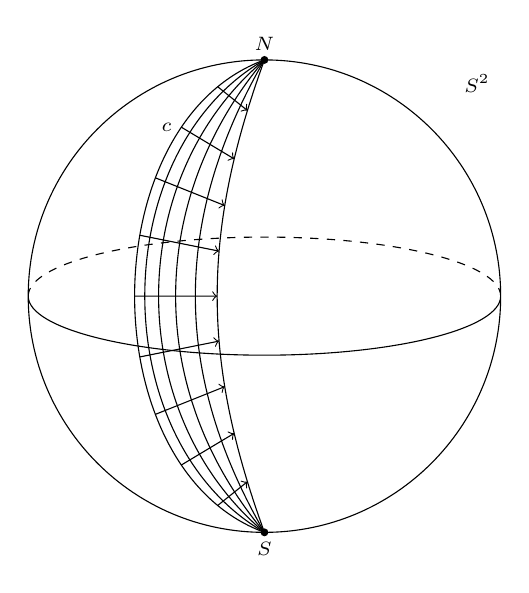
\begin{tikzpicture}[font=\scriptsize]
    % Kreis
    \def\radius{3}
    \draw (0,0) circle (\radius);
    % Ellipse
    \def\kleinradius{0.75}
    \begin{scope}
      \clip (-\radius,0) rectangle (\radius,1);
      \draw[dashed] (0,0) ellipse[x radius=\radius,y radius=\kleinradius];
    \end{scope}
    \begin{scope}
      \clip (-\radius,0) rectangle (\radius,-1);
      \draw (0,0) ellipse[x radius=\radius,y radius=\kleinradius];
    \end{scope}
    % Beschriftungen
    \coordinate (N) at (0,\radius); \coordinate (S) at (0,-\radius);
    \fill (N) circle (0.05) node[above]{$N$} (S) circle (0.05) node[below]{$S$};
    \node at (0.9*\radius,0.9*\radius) {$S^2$};
    % Boegen
    \def\firstangle{20}
    \draw (N) to[out=180+\firstangle,in=180-\firstangle] node[left,pos=0.2]{$c$} (S);
    \def\stepangle{10}
    \foreach \i in {1,2,...,5}{
      \draw (N) to[out=180 + \firstangle + \i * \stepangle,in=180-\firstangle - \i * \stepangle] (S);
    }
    \foreach \i in {0.1,0.2,...,0.9}{
      \path (N) to[out=180+\firstangle,in=180-\firstangle] coordinate[pos=\i] (a) (S);
      \path (N) to[out=180 + \firstangle + 5 * \stepangle,in=180-\firstangle - 5 * \stepangle] coordinate[pos=\i] (b) (S);
      \draw[->] (a) -- (b);
    }
  \end{tikzpicture}\end{center}


%%
%% Vorlesung <2013-1-18 Fri>
%% 

\begin{bew}
Nach Satz \ref{satz-9-5} ist jedes Jacobifeld $\calJ$ entlang $c$ mit $\calJ(0) = 0$ von der Gestalt $\calJ(t) = \difffrac[s=0]{}{s} \exp_p(t(\dot c(0) + s\calJ'(0))$, oder allgemein $\difffrac[s=0]{}{s} \exp_{\gamma(s)} (t(V(s) + sW(s)))$.
Es gilt dann
\begin{align*}
	\calJ(1) = \difffrac[s=0]{}{s} \exp_p (\dot c(0) + s \calJ'(0)) = \exp_{p*\dot{c}(0)} (\calJ'(0))
\end{align*}
Damit existiert genau dann ein nichttriviales Jacobifeld $\calJ$ entlang $c$ mit $\calJ(0) = 0$, $\calJ(1) = 0$, wenn $\Kern \exp_{p*\dot{c}(0)} \ne \{0\}$.
\end{bew}

\begin{bem}\begin{enumerate}[label=\arabic*),leftmargin=*]
\item
	Der Raum der nichttrivialen Jacobifelder mit verschwindenden Endpunkten entlang $c$ hat genau die Dimension $\ddim \Kern \exp_{p*\dot{c}(0)}$.
\item
	Ist $p$ konjugiert zu $q$, so ist $q$ konjugiert zu $p$.
\item
	F"ur jedes Jacobifeld $\calJ$ entlang $c$ mit $\calJ(0) = 0 = \calJ(1)$ gilt $\langle \calJ, \dot c \rangle = \langle \calJ', \dot c \rangle = 0$, denn
	\begin{align*}
		\langle \calJ', \dot c \rangle' = \langle \calJ'', \dot c \rangle = - \langle R(\calJ, \dot c) \dot c, \dot c \rangle = 0,
	\end{align*}
	also ist $\langle \calJ', \dot c \rangle = \langle \calJ, \dot c \rangle'$ konstant. Ferner gilt $\langle \calJ(0), \dot c (0) \rangle = 0 = \langle \calJ(1), \dot c(1) \rangle$, also ist $\langle \calJ, \dot c \rangle \equiv 0$.
\item
	Sind $p$ und $q$ nicht entlang $c$ zueinander konjugiert, dann ist jedes Jacobifeld $\calJ$ entlang $c$ eindeutig durch $\calJ(0)$ und $\calJ(1)$ bestimmt, denn sind $\calJ$ und $\tilde\calJ$ Jacobifelder mit identischen Randwerten, so ist $\calJ - \tilde\calJ$ ein Jacobifeld welches in den Endpunkten verschwindet.
\item
	Zwei Punkte sind genau dann konjugiert entlang der Geod"atischen $c$, wenn eine eigentliche geod"atische Variation von $c$ existiert.
\end{enumerate}\end{bem}

\begin{Satz}\label{satz-9-8}
Es seien $p, q \in M$ und sei $c: [0,1] \to M$ eine Geod"atische von $p$ nach $q$.\begin{enumerate}[label=(\roman*),widest=ii]
\item
	Ist entlang $c$ kein Punkt zu $p$ konjugiert, dann existiert eine Umgebung $U$ von $c$ in $\Omega_{pq}$, so dass $\calL(\tilde c) > \calL(c)$ und $E(\tilde c) \ge E(c)$ f"ur alle $\tilde c \in U$ gelten.
\item
	Falls ein $t_0 \in (0,1)$ existiert, so dass $p = c(0)$ zu $c(t_0)$ entlang $c$ konjugiert ist, so existiert eine eigentliche Variet"at $c_s$ von $c$ mit $\calL(c_s) < \calL(c)$ und $E(c_s) < E(c)$ f"ur hinreichend kleine $s$.
\end{enumerate}\end{Satz}

\begin{Lemma}[globales Gau"s Lemma]
Es seien $v, w \in \T_pM$ und $c(t) = \exp_p(t \cdot v)$. Dann gilt
\begin{align*}
	\langle \exp_{p*tv}(v), \exp_{p*tv}(w) \rangle = \langle v, w \rangle.
\end{align*}
Insbesondere ist jede Geod"atische in $p$ orthogonal zu der Abstandssph"are
\begin{align*}
	S_r(p) = \{ q | d(p, q) = r \}.
\end{align*}
\end{Lemma}

\begin{bew}
$Y$ sei das durch die Startwerte $Y(0) = 0$ und $Y'(0) = \frac{w}{t}$ bestimmte Jacobifeld entlang $c$. Dann gilt:
\begin{align*}
	Y(t) &= \difffrac[s=0]{}{s} \exp_{\gamma(s)}(t(V(s) + sW(s))) & \gamma(0) = p, \dot\gamma(0) = Y(0) = 0\\
	&= \difffrac[s=0]{}{s} \exp_p\left(t \left(v + s \frac{w}{t}\right)\right) & V(s) = V(0) = \dot c(0) = v\\
	&= \exp_{p*tv}(w) & W(s) = \ldots = \frac{w}{t}
\end{align*}
Es sei $\frac{w}{t} = \lambda v + u$ mit $u \perp v$. Der zu $c$ tangentiale Anteil von $Y$ ist dann
\begin{align*}
	Y^T(s) = \lambda s \dot c (s),
\end{align*}
denn ${Y^T}{''} = 0$ und $R(Y^T, \dot c) \dot c = \lambda s R(\dot c, \dot c) \dot c = 0$.
Also gilt $Y(t) = \lambda t \dot c(t) + Y^\perp(t)$, wobei $Y^\perp$ der zu $c$ orthogonale Anteil von $Y$ ist. Es folgt
\begin{align*}
	\langle \exp_{p*tv}(v), \exp_{p*tv}(w) \rangle &= \left\langle \difffrac{}{t} \smash{\underbrace{\exp_p(tv)}_{=c}}, Y(t) \right\rangle \vphantom{\underbrace{\difffrac{}{}}_{a}} \\
	&= \langle \dot c(t), \lambda t \dot c(t) + Y^\perp(t) \rangle \\
	&= \lambda t \|\dot c(t) \|^2 = \lambda t \|v\|^2 \\
\end{align*}
\begin{align*}
	\langle v, w \rangle &= \langle v, t(\lambda v + w) \rangle = t \lambda \|v\|^2
\end{align*}
\end{bew}

% Lemma 9.10
\begin{Lemma}\label{thm:lemma-9-10}
Es sei $c \colon [0,1] \to M$ eine Geodätische, $v = \dot c(0) \in \T_{p}M$ und $\psi$ (stückweise) glatte Kurve in $\T_pM$ mit $\psi(0) = 0$ und $\psi(1) = v$, dann gilt
\begin{align*}
	\mathcal L(\exp_p \circ \psi) \geq \mathcal L(c),
\end{align*}
wobei Gleichheit genau dann gilt, wenn $\psi$ eine monotone Reparametrisierung von $t \mapsto tv$ ist.
\end{Lemma}

\begin{bew}
Es seien $\rho$ und $\theta$ glatt, so dass $\psi = \rho \theta$ mit $\|\theta\| \equiv 1$ (Polarkoordinaten).
\begin{align*}
	\|(\exp_p \circ \psi)'\|^2 ={}& \|\exp_{p*\rho\theta} ( \rho' \theta + \rho \theta') \|^2 \\
	={}& {\rho'}{^2} \underbrace{\langle \exp_{p*\rho\theta} (\theta), \exp_{p*\rho\theta} (\theta) \rangle}_{= \langle \theta, \theta \rangle = 1} \\
	   & + 2\rho\rho' \underbrace{\langle \exp_{p*\rho\theta} (\theta), \exp_{p*\rho\theta} (\theta') \rangle}_{= \langle \theta, \theta' \rangle = \frac{1}{2} \|\theta\|^2{'} = 0} \\
	   & + \rho^2 \langle \exp_{p*\rho\theta} (\theta'), \exp_{p*\rho\theta} (\theta') \rangle \\
	={}& {\rho'}{^2} + \rho^2 \| \exp_{p*\psi}(\theta') \|^2
\end{align*}
Damit folgt
\begin{align*}
	\calL(\exp_p \circ \psi) \ge \int_0^1 | \rho' | \ge | \rho(1) - \rho(0) | = \|v\| = \calL(c)
\end{align*}
Gleichheit gilt genau dann, wenn $\theta$ konstant und $\rho$ monoton ist.
\end{bew}

\begin{bew}[von Satz \ref{satz-9-8}]\begin{enumerate}[label=(\roman*),leftmargin=*,widest=ii]
\item
	Es sei $c \colon [0,1] \to M$ eine Geodätische, seien $p = c(0)$ und $q = c(1)$ und es existieren keine zu $p$ konjugierten Punkte entlang $c$.
	Es bezeichne $\phi \colon [0,1] \to \T_pM$ mit $\phi(t) = tv$. Für jedes $t \in [0,1]$ ist nach Voraussetzung $\exp_{p*\phi(t)}$ regulär, also eine lokaler Diffeomorphismus.
	Es sei $\{W_i\}$ eine endliche offene Überdeckung von $\phi([0,1])$, so dass $\exp_p|_{W_i} \colon W_i \to \exp_p(W_i) = U_i$ ein Diffeomorphismus ist.
	
	\emph{Ziel:} Lifte Variationen von $M$ nach $\T_pM$.
	\begin{center}\begin{tikzpicture}[font=\scriptsize]
		%\tikzgitter{(-5,-5)}{(5,5)}
		
		\coordinate (a) at (-2.5,-1); \coordinate (b) at (3,2.5); % Endpkte. der Kurve
		\coordinate (ctrla) at (1,2); \coordinate (ctrlb) at (-2,-0.5); % Controls Punkte fuer die Kruemmung
		\coordinate (c) at ($(a) + (ctrla)$); \coordinate (d) at ($(b) + (ctrlb)$); % die daraus entstehenden Tangentialvektoren
		
		\draw (a) ..controls(c) and (d).. coordinate[pos=0.6] (beschr) (b); % die Hauptkurve
		\draw[->] (-0.5,2.5) node[left]{$c$} to[out=340,in=110] (beschr); % die Beschriftung
		
		\def\schlauchbreite{0.25cm}
		\def\schlauchweite{0.25cm}
		% Eckpunkte fuer den Schlauch, ueber- und unterhalb der Endpkte. und daneben
		\coordinate (0) at ($(a)!\schlauchbreite!90:(c)$); \coordinate (1) at ($(b)!\schlauchbreite!270:(d)$); \coordinate (2) at ($(b)!-\schlauchweite!0:(d)$);
		\coordinate (3) at ($(b)!\schlauchbreite!90:(d)$); \coordinate (4) at ($(a)!\schlauchbreite!270:(c)$); \coordinate (5) at ($(a)!-\schlauchweite!0:(c)$);
		% diese Vektoren geben die Verschiebung gegenueber den Endpktn. an
		\coordinate (shiftavert) at ($0.5*(0) - 0.5*(a)$); \coordinate (shiftbvert) at ($0.5*(1) - 0.5*(b)$);
		\coordinate (shiftahor) at ($0.5*(5) - 0.5*(a)$); \coordinate (shiftbhor) at ($0.5*(2) - 0.5*(b)$);
		%\draw[red] (0) circle(0.05) (1) circle(0.05) (2) circle(0.05) (3) circle(0.05) (4) circle(0.05) (5) circle(0.05);
		% der Schlauch
		\draw[dashed] (0) ..controls($(0) + (ctrla)$) and ($(1) + (ctrlb)$).. (1) ..controls($(1) + (shiftbhor)$) and ($(2) + (shiftbvert)$).. (2) ..controls($(2) - (shiftbvert)$) and ($(3) + (shiftbhor)$)..
			(3) ..controls($(3) + (ctrlb)$) and ($(4) + (ctrla)$).. (4) ..controls($(4) + (shiftahor)$) and($(5) - (shiftavert)$).. (5) ..controls($(5) + (shiftavert)$) and($(0) + (shiftahor)$).. (0) -- cycle;
		
		\draw[->] (4.5,3.5) node[right]{$\epsilon$-Schlauch} to[out=180,in=45] (1);
		
		\foreach \i in {0, 0.2, ...,1}{ % Kreise entlang der Kurve
			\path (a) ..controls(c) and (d).. coordinate[pos=\i] (p) (b);
			\draw (p) circle(0.8);
		}
		\node at (1,0.75) {$U_i$};
	\end{tikzpicture}\end{center}
	Es sei $t_i$ eine Partition von $[0,1]$, so dass $\phi([t_{i-1},t_i]) \subseteq W_i$. Ist $c_s$ eine Variation von $c$, so kann $\epsilon > 0$ so gewählt werden, dass
	\begin{align*}
		c_s \colon [t_{i-1},t_i]\X(-\epsilon,\epsilon) \to U_i = \exp_p(W_i)
	\end{align*}
	gilt. Dies definiert eine Variation $\psi_s$ von $\phi$ wie folgt:
	Ist $\psi_s$ bis $t_{i-1}$ definiert und gilt $\psi_s(t_{i-1}) \in W_i$, so setzt man $\psi_s(t) = \exp_p|_{W_i}^{-1}(c_s(t))$.
	Nach Lemma \ref{thm:lemma-9-10} gilt also
	\begin{align*}
		\mathcal L(\exp_p\circ \psi_s) = \mathcal L(c_s) \geq \mathcal L(c)
	\end{align*}
	für alle $s$. Mit der Cauchy-Schwarz Ungleichung folgt dann:
	\begin{align*}
		E(c_s) \geq \frac{1}{2} \mathcal L(c_s)^2 \geq \frac{1}{2} \mathcal
		L(c)^2 = E(c)
	\end{align*}
\item
	Es sei $c(t_0)$ entlang $c$ zu $p = c(0)$ konjugiert.
	
	\begin{description}\item[Behauptung:] Dann existiert ein zu $c$ orthogonales Vektorfeld $Y$ entlang der Geodätischen $c$ mit $Y(0) = 0$, $Y(1) = 0$ und $\calI(Y,Y) = 0$.\end{description}
	Dann gilt für die zugehärige eigentliche Variation $c_s$ von $c$:
	\begin{align*}
		\difffrac[s=0]{}{s}\mathcal L(c_s) = \lambda
		\difffrac[s=0]{}{s}E(c_s) = 0
	\end{align*}
	und, da $Y$ normal ist,
	\begin{align*}
		\difffrac[s=0]{^2}{s^2}\mathcal L(c_s) = \difffrac[s=0]{^2}{s^2}
		E(c_s) = \calI(Y,Y) < 0
	\end{align*}
	Somit ist $c$ lokales Maximum.
	\begin{description}\item[Beweis der Behauptung:]
		Es existiert ein nichttriviales (zu $c$ orthogonales) Jacobifeld $\calJ$ entlang $c|_{[0,t_0]}$ mit $\calJ(0) = 0$ und $\calJ(t_0) = 0$.
	\end{description}
\end{enumerate}\end{bew}

%%% Local Variables: 
%%% mode: latex
%%% TeX-master: "../skript-diffgeom"
%%% End: 